\documentclass[10pt]{beamer}\usepackage[]{graphicx}\usepackage[]{color}
% maxwidth is the original width if it is less than linewidth
% otherwise use linewidth (to make sure the graphics do not exceed the margin)
\makeatletter
\def\maxwidth{ %
  \ifdim\Gin@nat@width>\linewidth
    \linewidth
  \else
    \Gin@nat@width
  \fi
}
\makeatother

\definecolor{fgcolor}{rgb}{0.345, 0.345, 0.345}
\newcommand{\hlnum}[1]{\textcolor[rgb]{0.686,0.059,0.569}{#1}}%
\newcommand{\hlstr}[1]{\textcolor[rgb]{0.192,0.494,0.8}{#1}}%
\newcommand{\hlcom}[1]{\textcolor[rgb]{0.678,0.584,0.686}{\textit{#1}}}%
\newcommand{\hlopt}[1]{\textcolor[rgb]{0,0,0}{#1}}%
\newcommand{\hlstd}[1]{\textcolor[rgb]{0.345,0.345,0.345}{#1}}%
\newcommand{\hlkwa}[1]{\textcolor[rgb]{0.161,0.373,0.58}{\textbf{#1}}}%
\newcommand{\hlkwb}[1]{\textcolor[rgb]{0.69,0.353,0.396}{#1}}%
\newcommand{\hlkwc}[1]{\textcolor[rgb]{0.333,0.667,0.333}{#1}}%
\newcommand{\hlkwd}[1]{\textcolor[rgb]{0.737,0.353,0.396}{\textbf{#1}}}%
\let\hlipl\hlkwb

\usepackage{framed}
\makeatletter
\newenvironment{kframe}{%
 \def\at@end@of@kframe{}%
 \ifinner\ifhmode%
  \def\at@end@of@kframe{\end{minipage}}%
  \begin{minipage}{\columnwidth}%
 \fi\fi%
 \def\FrameCommand##1{\hskip\@totalleftmargin \hskip-\fboxsep
 \colorbox{shadecolor}{##1}\hskip-\fboxsep
     % There is no \\@totalrightmargin, so:
     \hskip-\linewidth \hskip-\@totalleftmargin \hskip\columnwidth}%
 \MakeFramed {\advance\hsize-\width
   \@totalleftmargin\z@ \linewidth\hsize
   \@setminipage}}%
 {\par\unskip\endMakeFramed%
 \at@end@of@kframe}
\makeatother

\definecolor{shadecolor}{rgb}{.97, .97, .97}
\definecolor{messagecolor}{rgb}{0, 0, 0}
\definecolor{warningcolor}{rgb}{1, 0, 1}
\definecolor{errorcolor}{rgb}{1, 0, 0}
\newenvironment{knitrout}{}{} % an empty environment to be redefined in TeX

\usepackage{alltt}%
\setbeamersize{text margin left=0.5cm, text margin right=0.5cm}

\usepackage{alltt}%
\usetheme[background=light]{metropolis} 
\usecolortheme{seahorse}

\usepackage[utf8]{inputenc}%


\usepackage[normalem]{ulem}%strikeout
 

% graphics
%% Figures %%%%%%%%%%%%%%%%%%%%%%%%%%%%%%%%%%%%%%%%%%%%%%%%%%
\usepackage{graphicx}
\usepackage{xcolor}%for color mixing

\usepackage{amsmath}%
\usepackage{amsfonts}%
\usepackage{amssymb}%
\usepackage{graphicx}

\usepackage{tikz}
\usetikzlibrary{calc}

\usepackage{hyperref}

%%%%%%%%%%%%%%%%%%%%%%%%%%%%%%%%%%%%%%%%%%%%%%
%%%%%%%%%%%%%%%%% Doc info %%%%%%%%%%%%%%%%%%%
\title{Introduction to R-Markdown}
\author{Timoth\'ee Bonnet}
\institute{BDSI / RSB}
\date{August 23, 2019}

%%%%%%%%%%%%%%%%%%%%%%%%%%%%%%%%%%%%
\IfFileExists{upquote.sty}{\usepackage{upquote}}{}
\begin{document}



\begin{frame}
\centering
\href{https://www.youtube.com/watch?v=s3JldKoA0zw}{
\includegraphics[width=0.8\textwidth]{Figures/markdownyoutube.png}}

\end{frame}
%%%%%%%%%%%

\begin{frame}
\maketitle
\end{frame}
%%%%%%%%%%%

\begin{frame}{Why use R-Markdown/Knitr}
\only<1>{
\centering
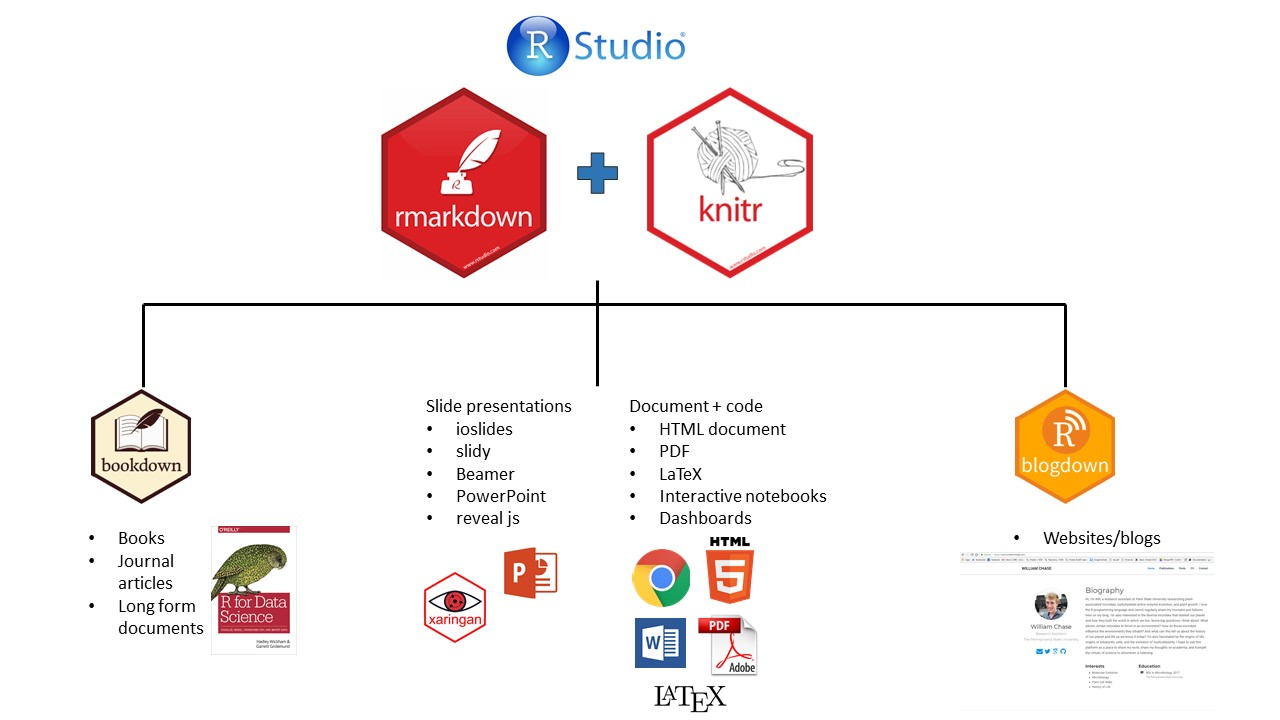
\includegraphics[width=0.9\textwidth]{Figures/rmarkdown_universe}
}
  \begin{itemize}
    \item Make your life easier
    \item Reproducible science
  \end{itemize}
\end{frame}
%%%%%%%%%%%


\begin{frame}{What you need:}

\begin{knitrout}\small
\definecolor{shadecolor}{rgb}{0.843, 0.867, 0.922}\color{fgcolor}\begin{kframe}
\begin{alltt}
\hlkwd{install.packages}\hlstd{(}\hlkwd{c}\hlstd{(}\hlstr{"knitr"}\hlstd{,} \hlstr{"xtable"}\hlstd{))}
\end{alltt}
\end{kframe}
\end{knitrout}

\end{frame}
%%%%%%%%%%%

\begin{frame}{Create an R Markdown html document in RStudio}
\centering
\only<1>{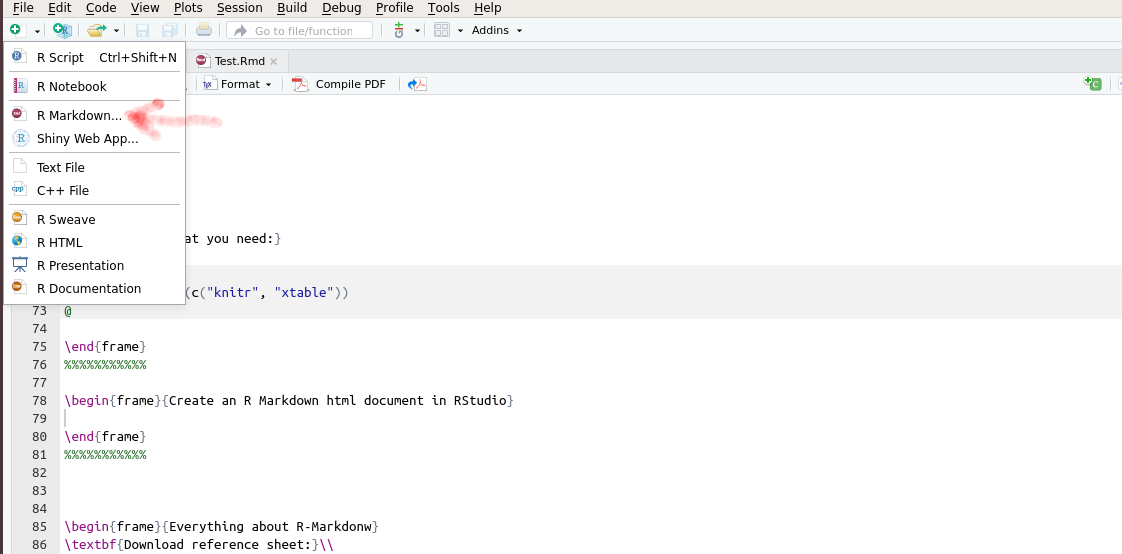
\includegraphics[width=0.8\textwidth]{Figures/Step1.png}}
\only<2>{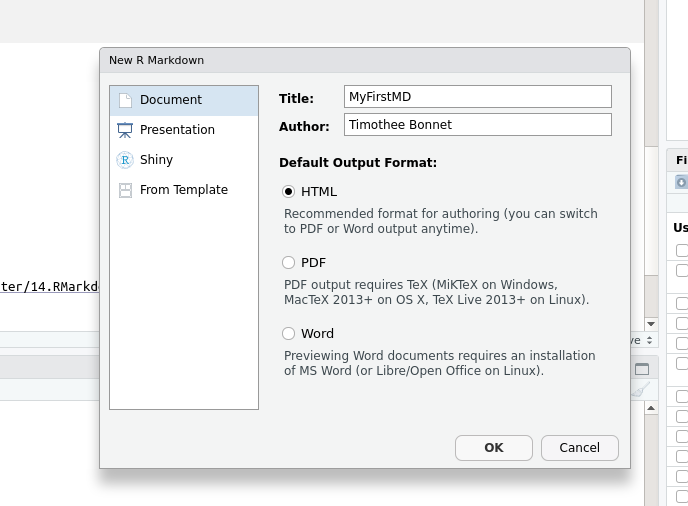
\includegraphics[width=0.8\textwidth]{Figures/Step2.png}}
\only<3>{

\begin{exampleblock}{Components of R-Markdown:}
  \begin{enumerate} 
    \item YAML = Configuration
    \item Text
    \item Code chunks
  \end{enumerate}
\end{exampleblock}

}
\end{frame}
%%%%%%%%%%%

\section{Text: Markdown syntax}

\begin{frame}{Text: Markdown syntax}
  \begin{columns}[t]
    \begin{column}{0.5\textwidth} 
      \uncover<1->{\texttt{Simple text}\\}
      \uncover<2->{\texttt{\# Header (main)} \\}
      \uncover<3->{\texttt{\#\# Header (section)} \\}
      \uncover<4->{\texttt{\#\#\# Header (sub-section)} \\}
      \uncover<5->{\texttt{*Italics*} \\}
      \uncover<6->{\texttt{**Bold**} \\}
      \uncover<7->{\texttt{Make a list:\\
                            - You can use\\
                            - asterisks (*)\\ 
                            - instead of -}\\}
            \vfill
    \end{column}
    \begin{column}{0.5\textwidth}
      \uncover<1->{Simple text\\}
      \uncover<2->{\textbf{\LARGE Header (main)} \\}
      \uncover<3->{\textbf{\Large Header (section)} \\}
      \uncover<4->{\textbf{\large Header (sub-section)} \\}
      \uncover<5->{\texttt{\textit{Italics}} \\}
      \uncover<6->{\texttt{\textbf{Bold}} \\}
      \uncover<7->{Make a list: \begin{itemize}
                    \item You can use
                    \item asterisks (*)
                    \item instead of -
                  \end{itemize}}
            \vfill
    \end{column}
\end{columns}
\end{frame}
%%%%%%%%%%%%%

\begin{frame}{Turn code into document: Compilation}
  \begin{itemize}
    \item Ctrl + Shift + K
    \item Click "Knit"\\
    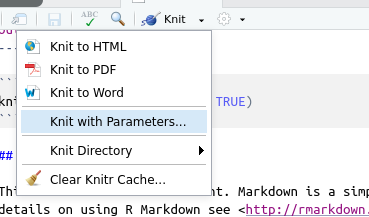
\includegraphics[width=0.5\textwidth]{Figures/knit}
  \end{itemize}
\end{frame}
%%%%%%%%%%%%%

\begin{frame}{Text: Exercise}

Create a new R Markdown document. Delete all of the R code chunks and write a bit of Markdown (some sections, some italicized text, and an itemized list).

Convert the document to a webpage.

\end{frame}
%%%%%%%%%%%

\begin{frame}{R-Code}

Insert a code chunk:
\begin{itemize}
  \item Ctrl+Alt+I
  \item Click \\
    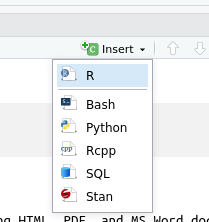
\includegraphics[width=0.35\textwidth]{Figures/chunk}
\end{itemize}
 
\end{frame}
%%%%%%%%%%%

\begin{frame}[fragile]{R-Code: Exercise}

\textbf{Insert the following code in your .Rmd document and compile it:}

\begin{knitrout}\small
\definecolor{shadecolor}{rgb}{0.843, 0.867, 0.922}\color{fgcolor}\begin{kframe}
\begin{alltt}
\hlstd{x1} \hlkwb{<-} \hlkwd{rnorm}\hlstd{(}\hlnum{200}\hlstd{)}
\hlstd{x2} \hlkwb{<-} \hlstd{x1} \hlopt{+}\hlkwd{rnorm}\hlstd{(}\hlnum{200}\hlstd{)}
\hlstd{y} \hlkwb{<-} \hlnum{1} \hlopt{+} \hlstd{x1} \hlopt{+}\hlkwd{rnorm}\hlstd{(}\hlnum{200}\hlstd{)}
\hlkwd{summary}\hlstd{(}\hlkwd{lm}\hlstd{(y} \hlopt{~} \hlstd{x2))}
\hlkwd{plot}\hlstd{(x2, y)}
\end{alltt}
\end{kframe}
\end{knitrout}

\end{frame}
%%%%%%%%%%%


\begin{frame}{Control chunk behavior:}
  \only<1>{\centering
  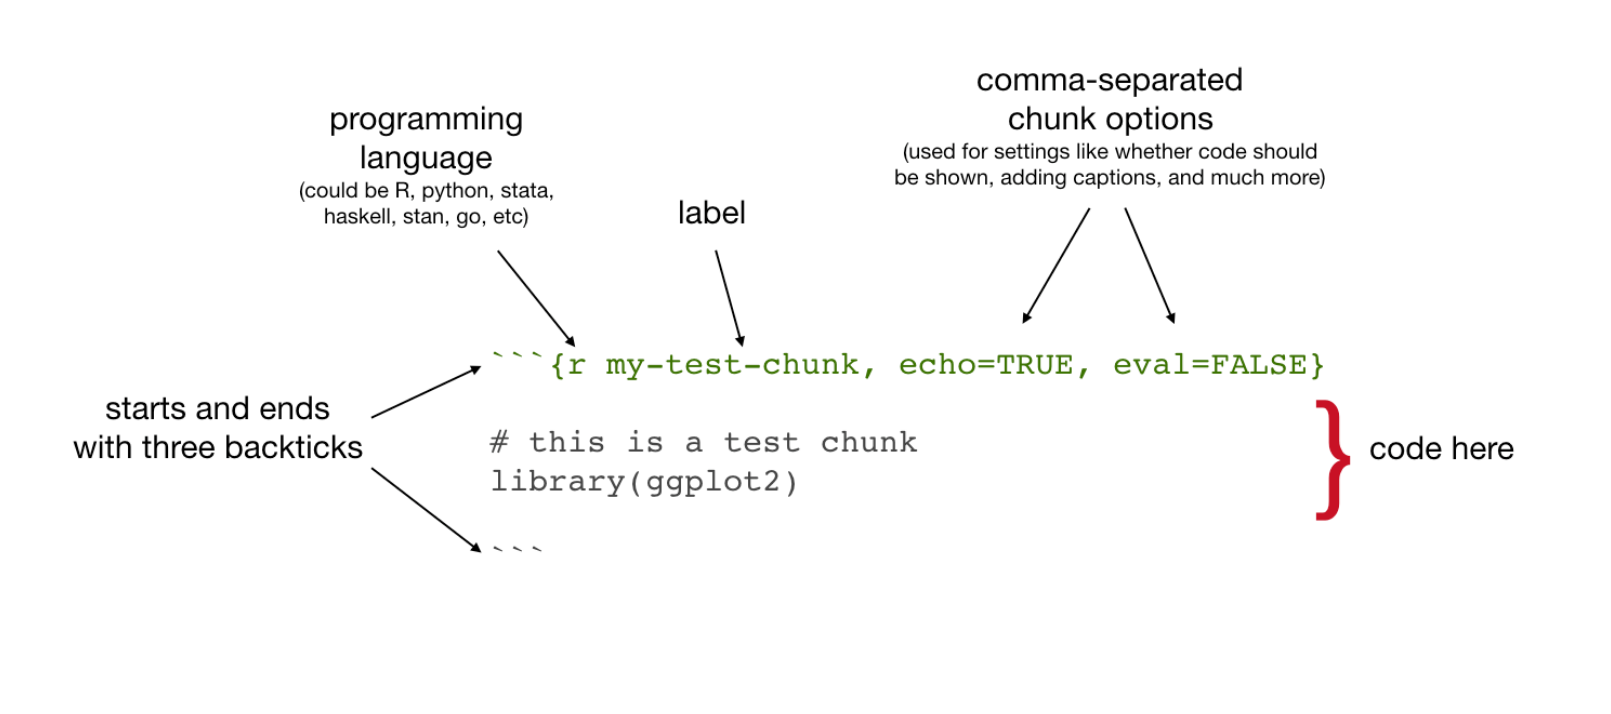
\includegraphics[width=\textwidth]{Figures/detailchunk}}
  \only<2>{
  Important options:
    \begin{itemize}
      \item echo= TRUE/FALSE ; show the code?
      \item eval= TRUE/FALSE ; run the code?
      \item collapse= TRUE/FALSE ; combine code and output?
      \item warning / message / error = TRUE/FALSE ; show what R wants to tell you?
      \item include = TRUE/FALSE ; show anything from the chunk in the document?
      \item fig.width / fig.height ; figure dimensions in inches
      \item fig.cap ; figure caption
      \item dev = 'pdf' / 'png' / 'svg' / 'jpeg' / 'tikz' /... ; How to create images?
    \end{itemize}
  }
\end{frame}
%%%%%%%%%%%%

\begin{frame}[fragile]{Inline R: make \textbf{every} number reproducible}
Try the two:

  \textbf{inline code displayed:}
\begin{knitrout}\small
\definecolor{shadecolor}{rgb}{0.843, 0.867, 0.922}\color{fgcolor}\begin{kframe}
\begin{alltt}
  \hlstd{` 1 + pi `}
\end{alltt}
\end{kframe}
\end{knitrout}
  
  \textbf{inline code output:}
\begin{knitrout}\small
\definecolor{shadecolor}{rgb}{0.843, 0.867, 0.922}\color{fgcolor}\begin{kframe}
\begin{alltt}
  \hlstd{`r 1 + pi `}
\end{alltt}
\end{kframe}
\end{knitrout}
  
\end{frame}
%%%%%%%%%%%

\section{A little bit of YAML}

\begin{frame}{YAML basics:}
\alert{Warning: YAML is very sensitive to spaces/tabs!}\\
\pause
Starts and end with 3 dashes
\pause
\begin{itemize}
  \item \texttt{title: "XX"}
  \item \texttt{author: "XX"}
  \item \texttt{date: "XX"}
  \item \texttt{output: html\_document / word\_document / pdf\_document } 
\end{itemize}
\end{frame}
%%%%%%%%%%%

\begin{frame}[fragile]{YAML options with html:}
Add a table of content (floating or fixed)
\begin{knitrout}\small
\definecolor{shadecolor}{rgb}{0.843, 0.867, 0.922}\color{fgcolor}\begin{kframe}
\begin{alltt}
\hlstd{output}\hlopt{:}
  \hlstd{html_document}\hlopt{:}
    \hlstd{toc}\hlopt{:} \hlstd{true}
    \hlstd{toc_float}\hlopt{:} \hlstd{true}
\end{alltt}
\end{kframe}
\end{knitrout}

\pause
Section numbering:
\begin{knitrout}\small
\definecolor{shadecolor}{rgb}{0.843, 0.867, 0.922}\color{fgcolor}\begin{kframe}
\begin{alltt}
\hlstd{output}\hlopt{:}
  \hlstd{html_document}\hlopt{:}
    \hlstd{number_sections}\hlopt{:} \hlstd{true}
\end{alltt}
\end{kframe}
\end{knitrout}

\end{frame}
%%%%%%%%%%%

\begin{frame}[fragile]{Html document look}

\textbf{theme:\\}
\texttt{default}, \texttt{cerulean}, \texttt{journal}, \texttt{flatly}, \texttt{darkly}, \texttt{readable}, \texttt{spacelab}, \texttt{united}, \texttt{cosmo}, \texttt{lumen}, \texttt{paper}, \texttt{sandstone}, \texttt{simplex}, and \texttt{yeti}. Pass \texttt{null} for no theme (in this case you can use the css parameter to add your own styles)

\pause

\textbf{highlight:\\}
\texttt{default}, \texttt{tango}, \texttt{pygments}, \texttt{kate}, \texttt{monochrome}, \texttt{espresso}, \texttt{zenburn}, \texttt{haddock}, \texttt{textmate} and \texttt{null}

\pause
\begin{knitrout}\small
\definecolor{shadecolor}{rgb}{0.843, 0.867, 0.922}\color{fgcolor}\begin{kframe}
\begin{alltt}
\hlstd{output}\hlopt{:}
  \hlstd{html_document}\hlopt{:}
    \hlstd{theme}\hlopt{:} \hlstd{united}
    \hlstd{highlight}\hlopt{:} \hlstd{tango}
\end{alltt}
\end{kframe}
\end{knitrout}

\end{frame}
%%%%%%%%%%%

\begin{frame}{YAML: Exercise}
  \begin{enumerate}
    \item Try compiling your Rmd as Word
    \item (If you have \LaTeX installed try compile as .pdf)
    \item Using HTML compilation add a table of content and change the theme
  \end{enumerate}
\end{frame}
%%%%%%%%%%%

\section{More markdown syntax}

\begin{frame}[fragile]{Insert pictures}

\begin{knitrout}\small
\definecolor{shadecolor}{rgb}{0.843, 0.867, 0.922}\color{fgcolor}\begin{kframe}
\begin{alltt}
![caption](Figures/markdown.png)
\end{alltt}
\end{kframe}
\end{knitrout}

or if you want more control with chunk options:

\begin{knitrout}\small
\definecolor{shadecolor}{rgb}{0.843, 0.867, 0.922}\color{fgcolor}\begin{kframe}
\begin{alltt}
```\{r, fig.cap=\hlstr{"R Markdown logo"}, fig.width=6\}
knitr::\hlkwd{include_graphics}(\hlstr{"Figures/markdown.jpg"})
```
\end{alltt}
\end{kframe}
\end{knitrout}


\end{frame}
%%%%%%%%%%%

\begin{frame}[fragile]{Insert hyperlink}
\begin{knitrout}\small
\definecolor{shadecolor}{rgb}{0.843, 0.867, 0.922}\color{fgcolor}\begin{kframe}
\begin{alltt}
[text to show](http://the-web-page.com)
\end{alltt}
\end{kframe}
\end{knitrout}
\end{frame}
%%%%%%%%%%%


\begin{frame}[fragile]{Insert tables}
Use the function kable in your .Rmd :

\begin{knitrout}\small
\definecolor{shadecolor}{rgb}{0.843, 0.867, 0.922}\color{fgcolor}\begin{kframe}
\begin{alltt}
\hlkwd{data}\hlstd{(cars)}
\hlstd{knitr}\hlopt{::}\hlkwd{kable}\hlstd{(}\hlkwc{x} \hlstd{=} \hlkwd{head}\hlstd{(cars),} \hlkwc{caption} \hlstd{=} \hlstr{"A knitr kable table"}\hlstd{)}
\end{alltt}
\end{kframe}
\end{knitrout}
\end{frame}
%%%%%%%%%%%

\begin{frame}[fragile]{Insert equations}
Follows \LaTeX format:\\

\textbf{Inline Math}

\begin{verbatim}
Hello $y_i = \mu + \beta \times x_i + \epsilon_i$, have a good day
\end{verbatim}

Hello $y_i = \mu + \beta \times x_i + \epsilon_i$, have a good day

\pause

\textbf{Equation Math}

\begin{verbatim}
Hello $$y_i = \mu + \beta \times x_i + \epsilon_i$$, have a good day
\end{verbatim}

Hello $$y_i = \mu + \beta \times x_i + \epsilon_i$$, have a good day

\end{frame}
%%%%%%%%%%%

\begin{frame}[fragile]{Insert tabs in html with \texttt{\{.tabset\}}}

\#\# Linear regression \{.tabset\}

\#\#\# Simple\\
A simple regression measures total associations

\begin{knitrout}\small
\definecolor{shadecolor}{rgb}{0.843, 0.867, 0.922}\color{fgcolor}\begin{kframe}
\begin{alltt}
```\{r\}
\hlkwd{summary}(\hlkwd{lm}(y ~ x2))
```
\end{alltt}
\end{kframe}
\end{knitrout}

\#\#\# Multiple\\
A multiple regression measures direct associations, corrected for indirect associations.
\begin{knitrout}\small
\definecolor{shadecolor}{rgb}{0.843, 0.867, 0.922}\color{fgcolor}\begin{kframe}
\begin{alltt}
```\{r\}
\hlkwd{summary}(\hlkwd{lm}(y ~ x1+x2))
```
\end{alltt}
\end{kframe}
\end{knitrout}
\end{frame}
%%%%%%%%%%%

%%%%%%%%%%%%%%%%%%%%%%%%%%%%%%%%%%%%%%%%%%%%%%%%%%%%%%%%%%%%%%%

\begin{frame}{Final exercise}

Turn the file "ToConvertToRMD.R" into a nice report/web-page
For instance:
\begin{itemize}
  \item Turn comments into text and equations
  \item Explain what the code is doing in text
  \item Add sections and table of content
  \item Print tables, figures (with captions!), inline numbers\dots
  \item Control the style
  \item Show or hide parts of the code (what goes in a report vs. just having a look at the data)
  \item Add iris pictures\dots
  \item \dots have fun!
\end{itemize}

\textbf{Use your own R code if you prefer!}

\end{frame}
%%%%%%%%%%%


\section{Conclusions}


\begin{frame}{Post-scriptum: Markdown or \LaTeX?}
Knitr can work with R-Markdonw (.Rmd files) and with Latex (.Rnw files)
\begin{itemize}
  \item Markdown is much simpler
  \item \LaTeX is much more flexible
  \item Pandoc let you translate a Markdown into Latex, then improve the Latex
\end{itemize}
\end{frame}
%%%%%%%%%%%

\begin{frame}{Cool things we haven't seen}
\begin{itemize}
  \item Add citations and make a bibliography (e.g., package citr)
  \item Cross-referencing
  \item Add non-R code (Python, Bash, SQL, stan...)
  \item How to make Slides (powerpoint, ioslides, beamer...)
  \item ...
\end{itemize}
\end{frame}
%%%%%%%%%%%

\begin{frame}{Everything about R-Markdonw}
\textbf{Download reference sheet:}\\
\url{https://github.com/timotheenivalis/RSB-R-Stats-Biology/raw/master/14.RMarkdown/rmarkdown-reference.pdf}

\textbf{Download quick cheatsheet:}\\
\url{https://github.com/timotheenivalis/RSB-R-Stats-Biology/raw/master/14.RMarkdown/rmarkdown-cheatsheet-2.0.pdf}

\textbf{More resources by RStudio:}\\
\url{https://rmarkdown.rstudio.com/index.html}

\end{frame}
%%%%%%%%%%%
\end{document}
